%%%%%%%%%%%%%%%%%%%%%%%%%%%%%%%%%%%%%%%%
% Class options                        %
%%%%%%%%%%%%%%%%%%%%%%%%%%%%%%%%%%%%%%%%
% Orientation:                         %
% portrait (default), landscape        %
%                                      %
% Paper size:                          %
% a0paper (default), a1paper, a2paper, %
% a3paper, a4paper, a5paper, a6paper   %
%                                      %
% Language:                            %
% english (default), norsk             %
%%%%%%%%%%%%%%%%%%%%%%%%%%%%%%%%%%%%%%%%
\documentclass{uioposter}


\usepackage{lipsum}                                % Dummy text
\usepackage[figwidth = 0.98\linewidth]{todonotes}  % Dummy image (and more!)
\usepackage[absolute, overlay]{textpos}            % Figure placement
\usepackage{adjustbox}
\usepackage{listings}
\usepackage{caption}
\setlength{\TPHorizModule}{\paperwidth}
\setlength{\TPVertModule}{\paperheight}


% colours for listings
\definecolor{keyword}{HTML}{2771a3}
\definecolor{pattern}{HTML}{b53c2f}
\definecolor{string}{HTML}{be681c}
\definecolor{relation}{HTML}{7e4894}
\definecolor{variable}{HTML}{107762}
\definecolor{comment}{HTML}{8d9094}

\lstset{
	numbers=none,
	stepnumber=1,
	numbersep=5pt,
	basicstyle=\small\ttfamily,
	keywordstyle=\color{keyword}\bfseries\ttfamily,
	commentstyle=\color{comment}\ttfamily,
	stringstyle=\color{string}\ttfamily,
	identifierstyle=\color{black},
	showstringspaces=false,
	aboveskip=3pt,
	belowskip=3pt,
	columns=flexible,
	keepspaces=true,
	breaklines=true,	
	captionpos=b,
	tabsize=2,
	frame=none
}

% Listing rules for Cypher

\lstdefinelanguage{cypher}
{
    morekeywords={
		MATCH, OPTIONAL, WHERE, NOT, AND, OR, XOR, RETURN, DISTINCT, ORDER, BY, ASC, ASCENDING, DESC, DESCENDING, UNWIND, AS, UNION, WITH, ALL, CREATE, DELETE, DETACH, REMOVE, SET, MERGE, SET, SKIP, LIMIT, IN, CASE, WHEN, THEN, ELSE, END, INDEX, DROP, UNIQUE, CONSTRAINT, EXPLAIN, PROFILE, START, CALL
	},
    ndkeywords={pageRank, iterate},
    keywordstyle={\color{keyword}\bfseries},
    ndkeywordstyle= {\color{relation}},
    sensitive=true
}

% Listing rules for Gremlin

\lstdefinelanguage{gremlin}
{
    keywordstyle = {\color{keyword}},
    morekeywords = {
        has, outE, order, by, desc, asc, inV, select, circle, gt, lt, leq, as, geoWithin, hasLabel, out, except, V, where, values, neq, eq, valueMap, limit, in, dedup, fold, unfold, inE, between, union, filter, get, value, atZone, of, getMonthValue, toLocalDate
    },
    ndkeywords={Geoshape, ZoneId},
    ndkeywordstyle= {\color{relation}},
    sensitive=true,
    morestring=*[d]{"},
}

% Listing rules for GSQL

\lstdefinelanguage{gsql}
{
	morekeywords={
		CREATE, QUERY, FOR, GRAPH, SELECT, FROM, WHERE, PRINT, ACCUM, INTERSECT, TYPEDEF, LIMIT, DO, FOREACH, RANGE, DO, IN, END, YEAR, MONTH
	},
	keywordstyle=\color{keyword}\bfseries,
	ndkeywords={SetAccum, ListAccum, HeapAccum, STRING, INT, DOUBLE, VERTEX, EDGE, tuple, DATETIME},
    ndkeywordstyle=\color{relation},
    sensitive=true,
    morestring=*[d]{"},
}


\lstset{
   extendedchars=true,
   basicstyle=\tiny\ttfamily,
   showstringspaces=false,
   showspaces=false,
   numberstyle=\footnotesize,
   numbersep=9pt,
   tabsize=2,
   breaklines=true,
   showtabs=false,
   captionpos=b
}


\title{An investigation into the suitability of graph database technology in the analysis of spatio-temporal data}
\author
{%
    S.D.~Baker Effendi\inst{1}
    \and
    A.B.~van der Merwe\inst{2}
}
%% Optional:
\institute
{
    Department of Computer Science, Stellenbosch University \\
    \texttt{dbe@sun.ac.za}\inst{1} \and \texttt{abvdm@cs.sun.ac.za}\inst{2}
}
% Or:
%\institute{Contact information}


%% Remove footline:
%\setbeamertemplate{footline}{}


\begin{document}
\begin{frame}
\begin{columns}[onlytextwidth]


\begin{column}{0.5\textwidth - 1.5cm}
    \begin{block}{Introduction}
        Large quantities of spatio-temporal data are captured everyday, whether by large web-based companies for social data or by other industries such as those concerning disaster relief or marine data analysis. This increases the need for backend systems to provide realtime query response times while scaling well (in terms of storage and performance) with increasing quantities of structured or semi-structured, multi-dimensional data. 
        
        \begin{figure}
            \centering
            
            
\includegraphics[width=.19\textwidth]{img/databases/postgreslogo.png}
            \hfill
            
\includegraphics[width=.2\textwidth]{img/databases/januslogo.png}
            \hfill
            
\includegraphics[width=.19\textwidth]{img/databases/tigergraph.png}
            \hfill
            
\includegraphics[width=.19\textwidth]{img/yelp-logo.png}
            
            \caption{The three databases; PostgreSQL, JanusGraph, and TigerGraph, and Yelp logo from which the dataset is obtained.}
            \label{fig:databases}
        \end{figure}
        
        Three database technologies will be investigated using this dataset namely: PostgreSQL, JanusGraph, and TigerGraph. The dataset used is the Yelp challenge dataset and the evaluation is based on how each database performs under data analysis scenarios similar to those found on an enterprise level.
    \end{block}

    % \begin{exampleblock}{Does it come in black?}
    %     Sure, use an \textbf{exampleblock}!
    % \end{exampleblock}

    % \begin{alertblock}{How do you make it pop?}
    %     Use an \alert{alertblock}!
    % \end{alertblock}

    \begin{block}{Implementation}
        Kernels represent ``real world'' data analysis and associated database operations(s). Due to the large amount of text data from the dataset's reviews, sentiment analysis is performed using NLTK\footnote{The Natural Language Toolkit. Written in Python. \url{www.nltk.org}.} to extract additional data and further motivate the application of each kernel.
        
        An Angular front-end/Flask back-end web application was written to schedule each job, call queries, and perform the data analysis. Each database and the web application was containerized using Docker.
        \begin{figure}
            \centering
            
            
\includegraphics[width=.20\textwidth]{img/webapp/angular-logo.png}
            \hfill
            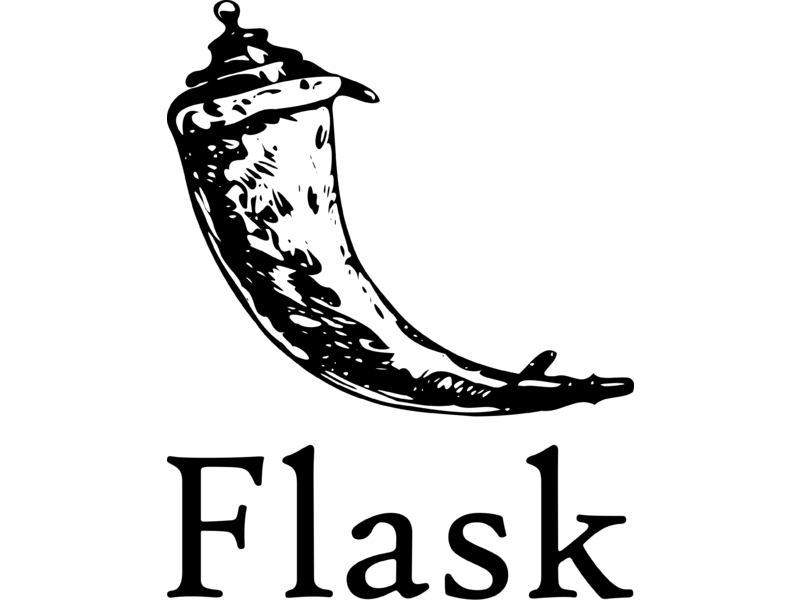
\includegraphics[width=.20\textwidth]{img/webapp/flask-logo.png}
            \hfill
            
\includegraphics[width=.18\textwidth]{img/webapp/nltk-logo.png}
            \hfill
            
\includegraphics[width=.20\textwidth]{img/webapp/docker-whale.png}
            
            \caption{The technologies used to implement each kernel, store results, and containerize the experiment environment.}
            \label{fig:webapp}
        \end{figure}
        
        Each kernel varies in complexity and adds some spatio-temporal constraint. These kernels were implemented on varying percentages of data from the dataset to investigate how each database handles increasing volumes of data.
        
        \medskip
        
    \end{block}
\end{column}


\begin{column}{0.5\textwidth - 1.5cm}
    \begin{block}{Graph Query Languages}
        Three graph query languages were considered during this investigation: Gremlin, Cypher, and GSQL. Examples of Gremlin and GSQL are shown below respectively:
        \begin{columns}
            \hspace{5pt}
            \begin{column}{.49\textwidth}
                \lstinputlisting[
                language=gremlin]
                {./queries/kate.groovy}
            \end{column}%
            \begin{column}{.49\textwidth}
                \lstinputlisting[
                language=gsql]
                {./queries/kate.gsql}
            \end{column}%
        \end{columns}
        Each graph query traversal language has varying degrees of capability, expressiveness, and conciseness. These graph traversal languages are designed to express graph pattern matches in an effective way.
    \end{block}

    \begin{block}{Results}
        The results suggest that the mean query response time of graph databases scale much better than relational databases. PostgreSQL does not handle complex, spatio-temporal queries as well as JanusGraph and TigerGraph do.
        \begin{figure}
            \centering
            
            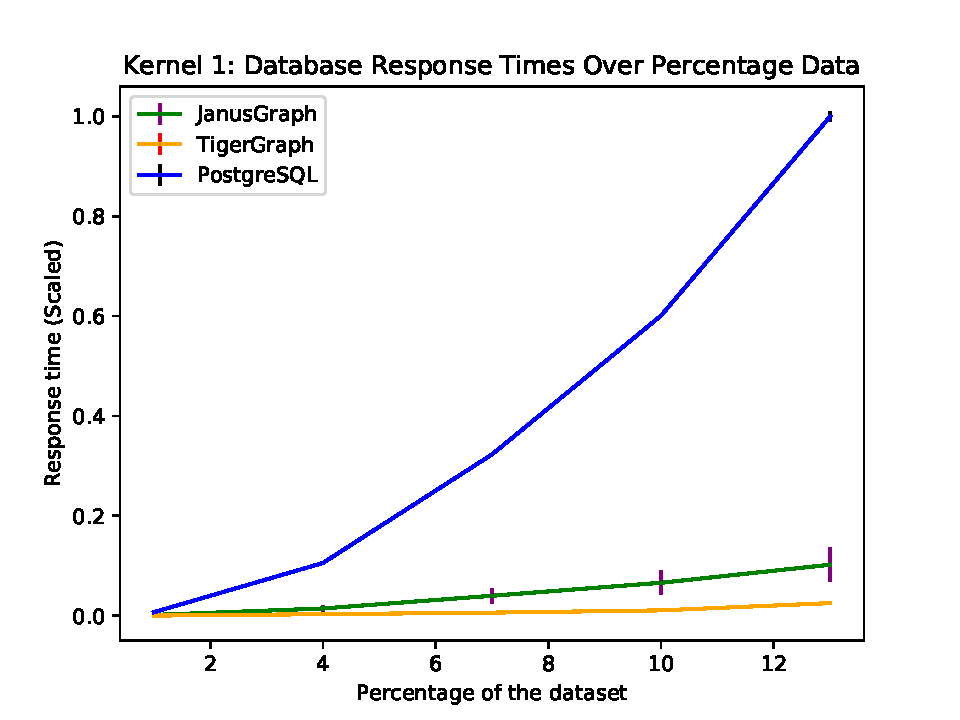
\includegraphics[width=.49\textwidth]{img/results/katePlotSetup1.pdf}
            \hfill
            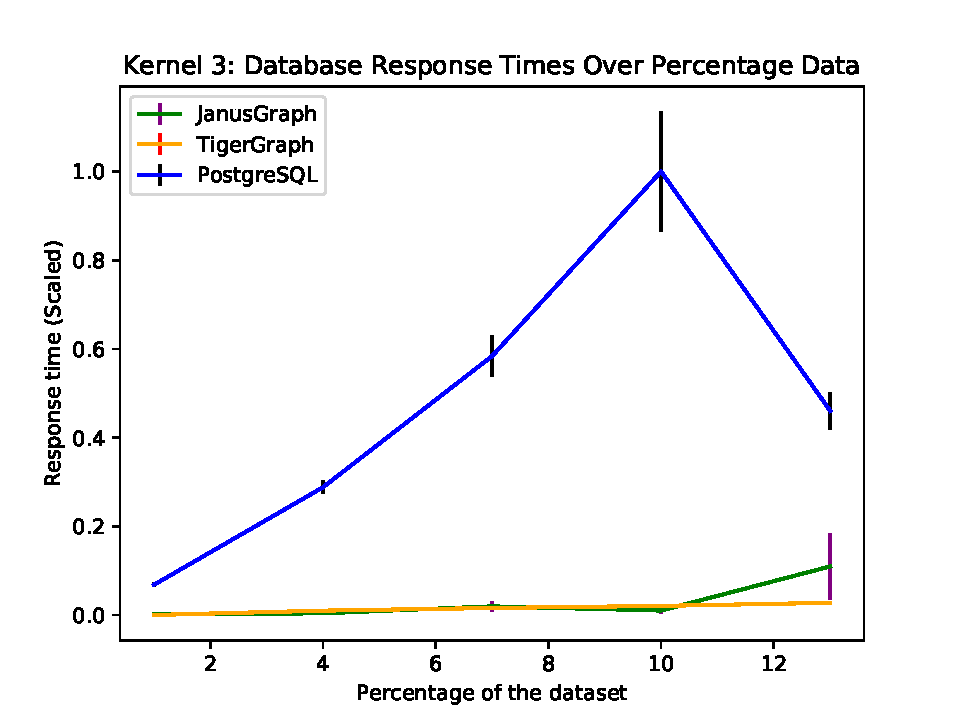
\includegraphics[width=.49\textwidth]{img/results/cityPlotSetup1.pdf}
            
            \caption{The results of two kernels over varying volumes of the dataset.}
            \label{fig:results}
        \end{figure}
    \end{block}

    \begin{block}{Conclusion}
        This investigation demonstrated that:
        \vfill
        \begin{itemize}
            \item For complex, spatio-temporal queries our two graph databases were \textbf{superior} to our relational database in terms of query response times
            \item Graph query languages are often \textbf{more concise or expressive} than SQL when writing graph traversals
            \item Graph databases are indeed \textbf{suitable} for use in the \textbf{analysis of spatio-temporal data}
        \end{itemize}
    \end{block}
\end{column}


\end{columns}


\begin{textblock}{0.5}(0.14, 0.95)
    \color{white}
    \sffamily
    \small
    \textbf{Stellenbosch University}
    \\
    Stellenbosch 7600, South Africa
\end{textblock}


\end{frame}
\end{document}